\section{Преобразование Фурье}

Рассмотрим унитарное преобразование Фурье к угловой частоте $\omega$:
\begin{equation}
    \hat{f}(\omega) = \frac{1}{\sqrt{2\pi}} \int_{-\infty}^{\infty} f(t) e^{-i\omega t} dt
    \label{eq:image_from_function}
\end{equation}

Обратное преобразование Фурье:
\begin{equation}
    f(t) = \frac{1}{\sqrt{2\pi}} \int_{-\infty}^{\infty} \hat{f}(\omega) e^{i\omega t} d\omega
    \label{eq:function_from_image}
\end{equation}

Равенство Парсеваля:
\begin{equation}
    \int_{-\infty}^{\infty} |f(t)|^2 dt = \int_{-\infty}^{\infty} |\hat{f}(\omega)|^2 d\omega
    \label{eq:parseval_indentity}
\end{equation}


\section{Вещественные функции}
\subsection{Прямоугольная функция}

Рассмотрим семейство функций 
\begin{equation}
    f(t) = \begin{cases}
        a, & |t| \le b, \\
        0, & |t| > b
    \end{cases}
    \label{eq:rectangle_function}
\end{equation}

\subsubsection{Графики исходных функций}
Графики данной функции при различных значениях $a$ и $b$ представлены на рисунках \ref{fig:rectangle_1}, \ref{fig:rectangle_2} и \ref{fig:rectangle_3}.

\begin{figure}[ht!]
    \centering
    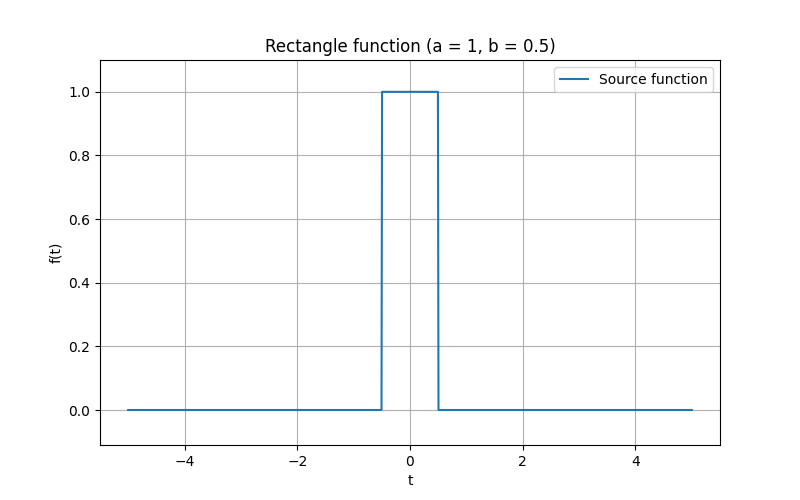
\includegraphics[width=\textwidth]{media/rectangle_1.png}
    \caption{График прямоугольной функции $f(t)$ при $a = 1$, $b = 0.5$}
    \label{fig:rectangle_1}
\end{figure}

\begin{figure}[ht!]
    \centering
    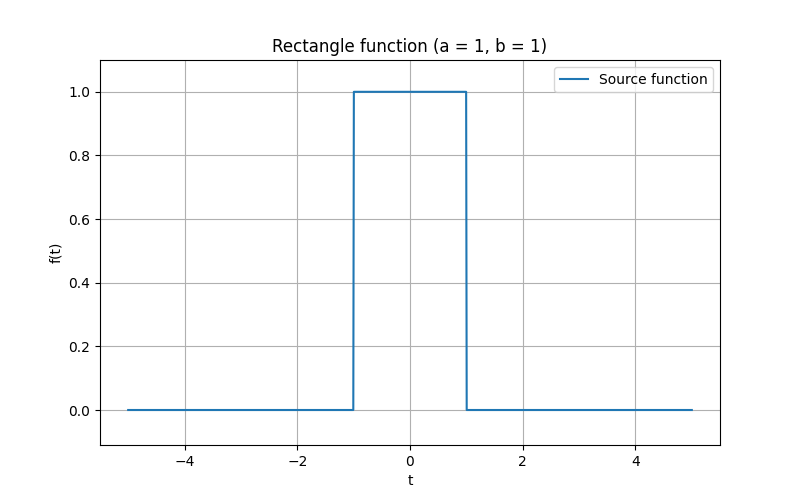
\includegraphics[width=\textwidth]{media/rectangle_2.png}
    \caption{График прямоугольной функции $f(t)$ при $a = 1$, $b = 1$}
    \label{fig:rectangle_2}
\end{figure}

\begin{figure}[ht!]
    \centering
    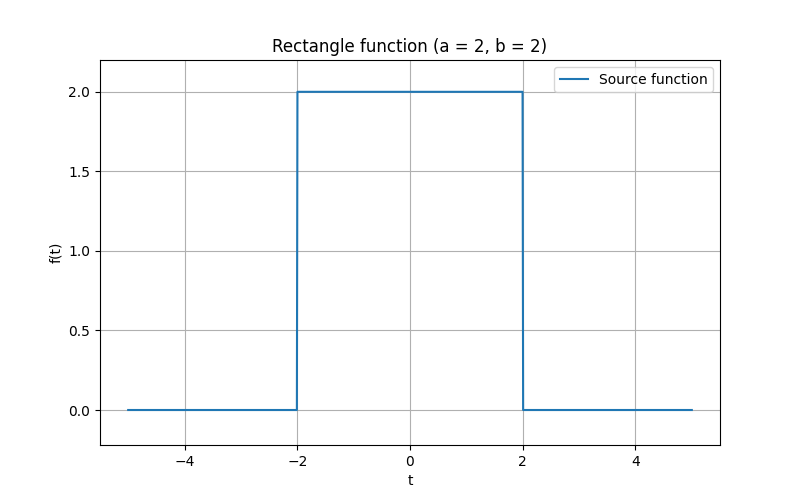
\includegraphics[width=\textwidth]{media/rectangle_3.png}
    \caption{График прямоугольной функции $f(t)$ при $a = 2$, $b = 2$}
    \label{fig:rectangle_3}
\end{figure}

\subsubsection{Нахождение образа функции}
Согласно формуле \eqref{eq:image_from_function}, Фурье образ функции $f(t)$ задается следующим выражением:
\begin{equation}
    \hat{f}(\omega) = \frac{1}{\sqrt{2\pi}} \int_{-\infty}^{\infty} f(t) e^{-i\omega t} dt = \frac{1}{\sqrt{2\pi}} \int_{-b}^{b} a e^{-i\omega t} dt = \frac{a}{-\omega i\sqrt{2\pi}} e^{-i\omega t} \Biggr|_{-b}^{b} = \frac{a(e^{i\omega b} - e^{-i\omega b})}{\omega i \sqrt{2 \pi}}
\end{equation}

Применив формулу Эйлера, получим:
\begin{equation}
    \hat{f}(\omega) = \frac{2ab}{\sqrt{2\pi}}\sinc(\omega b)
    \label{eq:rectangle_image}
\end{equation}

для $a = 1$, $b = 0.5$:
\begin{equation}
    \hat{f_1}(\omega) = \frac{1}{\sqrt{2\pi}}\sinc(\omega / 2)
\end{equation}

для $a = 1$, $b = 1$:
\begin{equation}
    \hat{f_2}(\omega) = \frac{2}{\sqrt{2\pi}}\sinc(\omega)
\end{equation}

для $a = 2$, $b = 2$:
\begin{equation}
    \hat{f_3}(\omega) = \frac{8}{\sqrt{2\pi}}\sinc(2\omega)
\end{equation}

\subsubsection{Графики образов функций}
Графики образов прямоугольной функции при различных значениях $a$ и $b$ представлены на рисунках \ref{fig:rectangle_1_image}, \ref{fig:rectangle_2_image} и \ref{fig:rectangle_3_image}.

\begin{figure}[ht!]
    \centering
    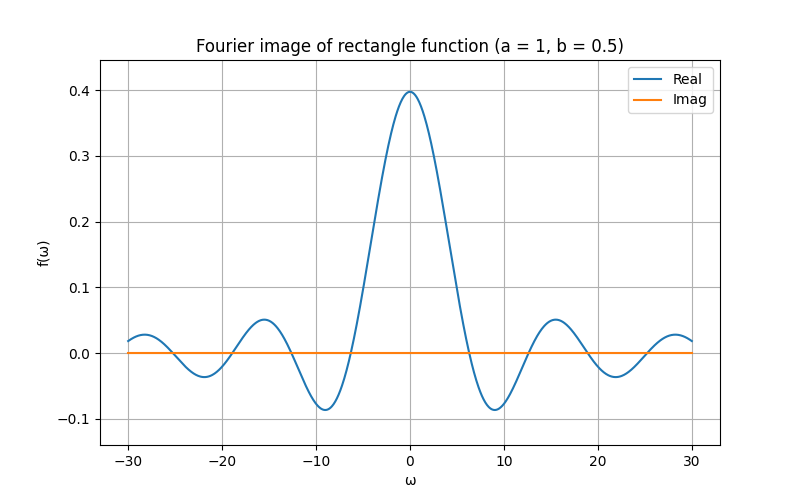
\includegraphics[width=\textwidth]{media/rectangle_1_image.png}
    \caption{График преобразования Фурье $\hat{f_1}(\omega)$ прямоугольной функции $f(t)$ при $a = 1$, $b = 0.5$}
    \label{fig:rectangle_1_image}
\end{figure}

\begin{figure}[ht!]
    \centering
    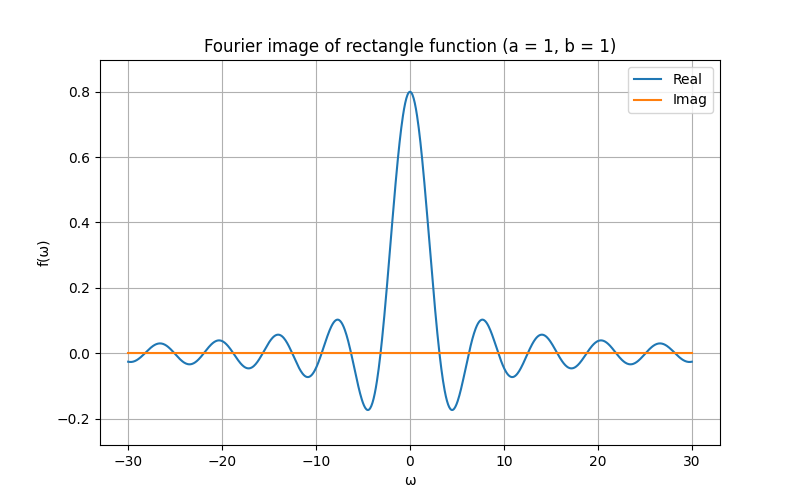
\includegraphics[width=\textwidth]{media/rectangle_2_image.png}
    \caption{График преобразования Фурье $\hat{f_2}(\omega)$ прямоугольной функции $f(t)$ при $a = 1$, $b = 1$}
    \label{fig:rectangle_2_image}
\end{figure}

\begin{figure}[ht!]
    \centering
    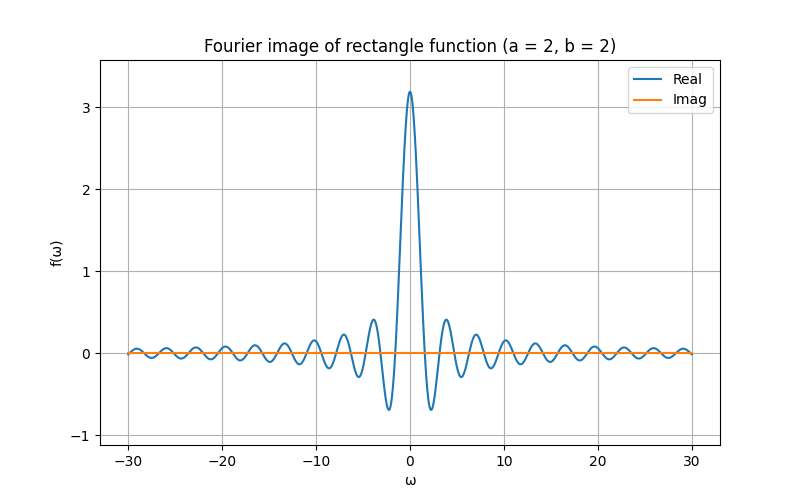
\includegraphics[width=\textwidth]{media/rectangle_3_image.png}
    \caption{График преобразования Фурье $\hat{f_3}(\omega)$ прямоугольной функции $f(t)$ при $a = 2$, $b = 2$}
    \label{fig:rectangle_3_image}
\end{figure}

\FloatBarrier
\subsubsection{Проверка равенства Парсеваля}
Проверим равенство Парсеваля (см. формулу~\eqref{eq:parseval_indentity}). Для этого воспользуемся функцией \texttt{parseval\_check}. 
% table with parseval check results
\begin{table}[ht!]
    \centering
    \begin{tabular}{|c|c|}
        \hline
        $\displaystyle\int_{-100}^{100}{|f(t)|^2}$ & $\displaystyle\int_{-100}^{100}{|\hat{f_1}(\omega)|^2}$ \\
        \hline
        1.00010 & 0.99376 \\
        \hline
    \end{tabular}
    \caption{Результаты проверки равенства Парсеваля для прямоугольной функции $f(t)$ при $a = 1$, $b = 0.5$}
    \label{tab:rectangle_1_parseval_check}
\end{table}

\begin{table}[ht!]
    \centering
    \begin{tabular}{|c|c|}
        \hline
        $\displaystyle\int_{-100}^{100}{|f(t)|^2}$ & $\displaystyle\int_{-100}^{100}{|\hat{f_2}(\omega)|^2}$ \\
        \hline
        2.00020 & 1.99386 \\
        \hline
    \end{tabular}
    \caption{Результаты проверки равенства Парсеваля для прямоугольной функции $f(t)$ при $a = 1$, $b = 1$}
    \label{tab:rectangle_2_parseval_check}
\end{table}

\begin{table}[ht!]
    \centering
    \begin{tabular}{|c|c|}
        \hline
        $\displaystyle\int_{-100}^{100}{|f(t)|^2}$ & $\displaystyle\int_{-100}^{100}{|\hat{f_3}(\omega)|^2}$ \\
        \hline
        16.00160 & 15.97619 \\
        \hline
    \end{tabular}
    \caption{Результаты проверки равенства Парсеваля для прямоугольной функции $f(t)$ при $a = 2$, $b = 2$}
    \label{tab:rectangle_3_parseval_check}
\end{table}

Видим, что во всех случаях значения почти не отличаются друг от друга. Различие, по большей части, обусловлено тем, что в программе нельзя найти интеграл по бесконечности, поэтому просто берется достаточно большой интервал интегрирования.

\subsubsection{Анализ результатов}
Влияние параметров $a$ и $b$ на графики прямоугольной функции и ее образа можно понять из соответствующих формул (см. формулы~\eqref{eq:rectangle_function} и~\eqref{eq:rectangle_image}).
В исходной функции $f(t)$ параметр $a$ отвечает за высоту прямоугольника, а $b$ за его ширину.
В образе $\hat{f}(\omega)$ параметр $a$ отвечает за амплитуду колебаний, а $b$ за частоту колебаний.

Принцип неопределенности Гейзенберга утверждает, что нельзя одновременно точно определить положение и импульс частицы. В данном случае, чем меньше ширина прямоугольника, тем больше ширина его образа, и наоборот. 

\FloatBarrier

\subsection{Треугольная функция}

Рассмотрим семейство функций
\begin{equation}
    f(t) = \begin{cases}
        a - |at / b|, & |t| \le b, \\
        0, & |t| > b
    \end{cases}
    \label{eq:triangle_function}
\end{equation}

\subsubsection{Графики исходных функций}

\begin{figure}[ht!]
    \centering
    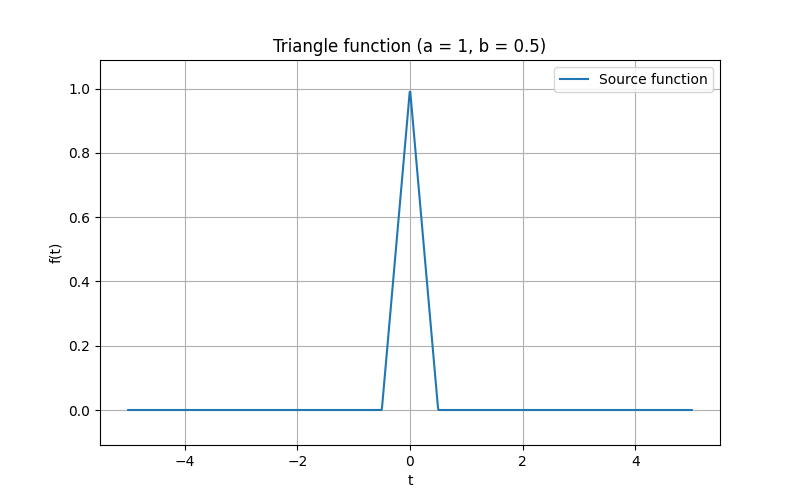
\includegraphics[width=\textwidth]{media/triangle_1.png}
    \caption{График прямоугольной функции $f(t)$ при $a = 1$, $b = 0.5$}
    \label{fig:triangle_1}
\end{figure}

\begin{figure}[ht!]
    \centering
    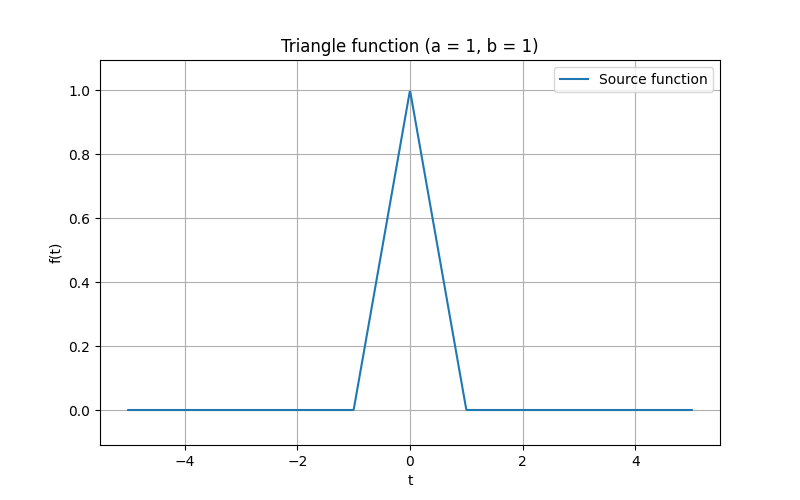
\includegraphics[width=\textwidth]{media/triangle_2.png}
    \caption{График прямоугольной функции $f(t)$ при $a = 1$, $b = 1$}
    \label{fig:triangle_2}
\end{figure}

\begin{figure}[ht!]
    \centering
    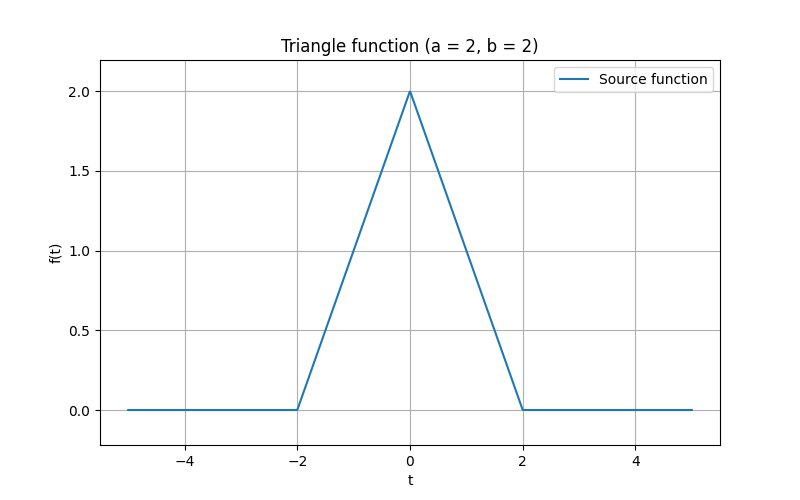
\includegraphics[width=\textwidth]{media/triangle_3.png}
    \caption{График прямоугольной функции $f(t)$ при $a = 2$, $b = 2$}
    \label{fig:triangle_3}
\end{figure}

\subsubsection{Нахождение образа функции}
Согласно формуле \eqref{eq:image_from_function}, Фурье образ функции $f(t)$ задается следующим выражением:
\begin{multline}
    \hat{f}(\omega) = \frac{1}{\sqrt{2\pi}} \int_{-\infty}^{\infty} f(t) e^{-i\omega t} dt = \frac{1}{\sqrt{2\pi}} \int_{-b}^{b} (a - |at / b|) e^{-i\omega t} dt = \\
    \frac{1}{\sqrt{2\pi}} \left(\int_{-b}^{0}{(a + \frac{at}{b}) e^{-i\omega t}} dt + \int_{0}^{b}{(a - \frac{at}{b}) e^{-i\omega t}} dt\right) =
    \frac{1}{\sqrt{2 \pi}} \left(\frac{a(ib\omega - e^{ib\omega} + 1)}{b \omega^2} + \frac{a(-ib\omega - e^{-ib\omega} + 1)}{b\omega^2} \right) = \\
    \frac{1}{\sqrt{2\pi}} \left( \frac{a (-e^{ib\omega} - e^{-ib\omega} + 2)} {b\omega^2} \right) = \frac{1}{\sqrt{2\pi}} \frac{4a \sin(\frac{b\omega}{2})^2}{b \omega^2}  = \frac{4a\sin(\frac{b\omega}{2})^2}{\sqrt{2\pi} b \omega^2} = \frac{ab}{\sqrt{2\pi}} \sinc^2\left(\frac{b\omega}{2}\right)
    \label{eq:truangle_image}
\end{multline}

для $a = 1$, $b = 0.5$:
\begin{equation}
    \hat{f_1}(\omega) = \frac{1}{\sqrt{2\pi}} \sinc^2\left(\frac{\omega}{4}\right)
\end{equation}

для $a = 1$, $b = 1$:
\begin{equation}
    \hat{f_2}(\omega) = \frac{1}{\sqrt{2\pi}} \sinc^2\left(\frac{\omega}{2}\right)
\end{equation}

для $a = 2$, $b = 2$:
\begin{equation}
    \hat{f_3}(\omega) = \frac{4}{\sqrt{2\pi}} \sinc^2\left(\omega\right)
\end{equation}

\subsubsection{Графики образов функций}
Графики образов треугольной функции при различных значениях $a$ и $b$ представлены на рисунках \ref{fig:triangle_1_image}, \ref{fig:triangle_2_image} и \ref{fig:triangle_3_image}.

\begin{figure}[ht!]
    \centering
    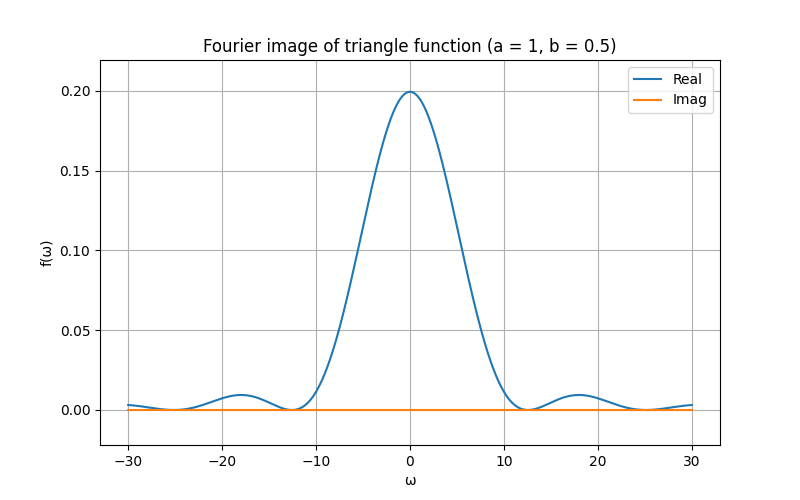
\includegraphics[width=\textwidth]{media/triangle_1_image.png}
    \caption{График Фурье образа треугольной функции $\hat{f}(\omega)$ при $a = 1$, $b = 0.5$}
    \label{fig:triangle_1_image}
\end{figure}

\begin{figure}[ht!]
    \centering
    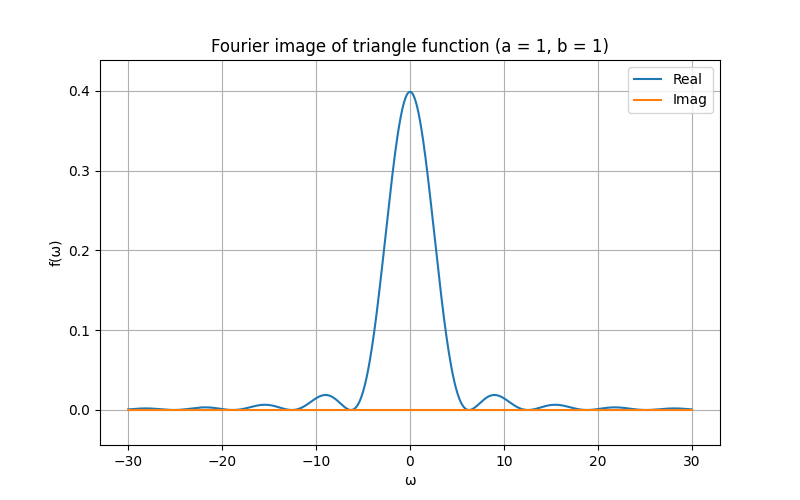
\includegraphics[width=\textwidth]{media/triangle_2_image.png}
    \caption{График Фурье образа треугольной функции $\hat{f}(\omega)$ при $a = 1$, $b = 1$}
    \label{fig:triangle_2_image}
\end{figure}

\begin{figure}[ht!]
    \centering
    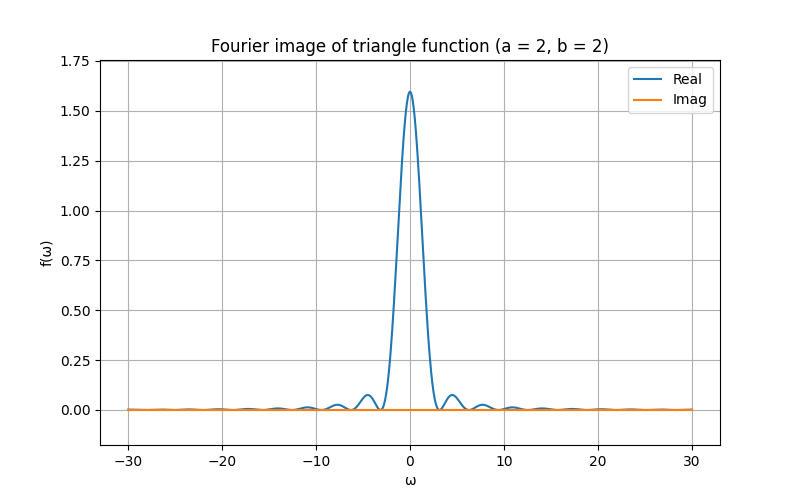
\includegraphics[width=\textwidth]{media/triangle_3_image.png}
    \caption{График Фурье образа треугольной функции $\hat{f}(\omega)$ при $a = 2$, $b = 2$}
    \label{fig:triangle_3_image}
\end{figure}

\FloatBarrier
\subsubsection{Проверка равенства Парсеваля}
Проверим равенство Парсеваля (см. формулу~\eqref{eq:parseval_indentity}). Для этого воспользуемся функцией \texttt{parseval\_check}.
\begin{table}[ht!]
    \centering
    \begin{tabular}{|c|c|}
        \hline
        $\displaystyle\int_{-100}^{100}{|f(t)|^2}$ & $\displaystyle\int_{-100}^{100}{|\hat{f_1}(\omega)|^2}$ \\
        \hline
        0.3333 & 0.3333 \\
        \hline
    \end{tabular}
    \caption{Результаты проверки равенства Парсеваля для треугольной функции $f(t)$ при $a = 1$, $b = 0.5$}
    \label{tab:triangle_1_parseval_check}
\end{table}

\begin{table}[ht!]
    \centering
    \begin{tabular}{|c|c|}
        \hline
        $\displaystyle\int_{-100}^{100}{|f(t)|^2}$ & $\displaystyle\int_{-100}^{100}{|\hat{f_2}(\omega)|^2}$ \\
        \hline
        0.6666 & 0.6666 \\
        \hline
    \end{tabular}
    \caption{Результаты проверки равенства Парсеваля для треугольной функции $f(t)$ при $a = 1$, $b = 1$}
    \label{tab:triangle_2_parseval_check}
\end{table}

\begin{table}[ht!]
    \centering
    \begin{tabular}{|c|c|}
        \hline
        $\displaystyle\int_{-100}^{100}{|f(t)|^2}$ & $\displaystyle\int_{-100}^{100}{|\hat{f_3}(\omega)|^2}$ \\
        \hline
        5.3333 & 5.3333 \\
        \hline
    \end{tabular}
    \caption{Результаты проверки равенства Парсеваля для треугольной функции $f(t)$ при $a = 2$, $b = 2$}
    \label{tab:triangle_3_parseval_check}
\end{table}

Видим, что во всех случаях равенство Парсеваля выполняется с высокой точностью.

\subsubsection{Анализ результатов}
Влияние параметров $a$ и $b$ на исходную функцию и ее Фурье образ определяются из формулы \eqref{eq:triangle_function} и выражения для Фурье образа \eqref{eq:truangle_image}. Параметр $a$ определяет высоту треугольной функции, а параметр $b$ --- ширину основания. В образе функции видно, что при увеличении параметра $a$ амплитуда образа увеличивается, а при увеличении параметров $a$ и $b$ амплитуда увеличивается, при увеличении параметра $b$ увеличивается частота. 

Принцип неопределенности, как и с прошлом случае, можно наблюдать как уменьшение ширины образа при увеличении основания треугольника.
\FloatBarrier

\subsection{Кардинальный синус}

Рассмотрим семейство функций
\begin{equation}
    f(t) = a \sinc(bt)
    \label{eq:sinc_function}
\end{equation}

\subsubsection{Графики исходных функций}
Графики данной функции при различных значениях $a$ и $b$ представлены на рисунках \ref{fig:sinc_1}, \ref{fig:sinc_2} и \ref{fig:sinc_3}.

\begin{figure}[ht!]
    \centering
    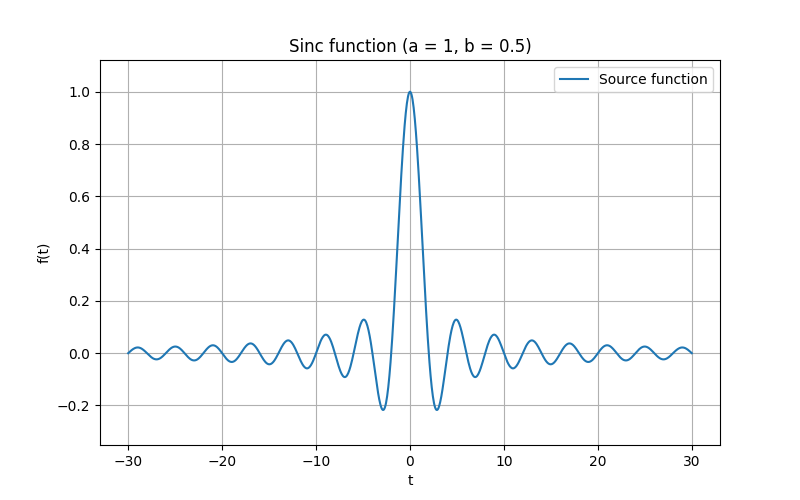
\includegraphics[width=\textwidth]{media/sinc_1.png}
    \caption{График функции $f(t)$ при $a = 1$, $b = 0.5$}
    \label{fig:sinc_1}
\end{figure}

\begin{figure}[ht!]
    \centering
    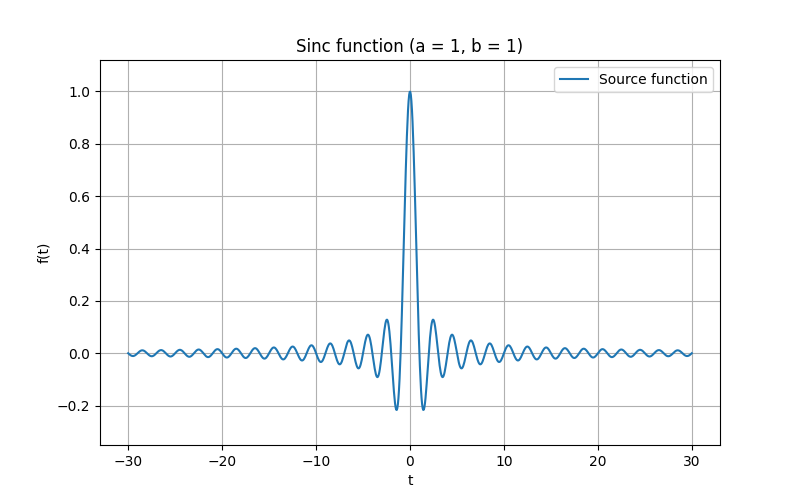
\includegraphics[width=\textwidth]{media/sinc_2.png}
    \caption{График функции $f(t)$ при $a = 1$, $b = 1$}
    \label{fig:sinc_2}
\end{figure}

\begin{figure}[ht!]
    \centering
    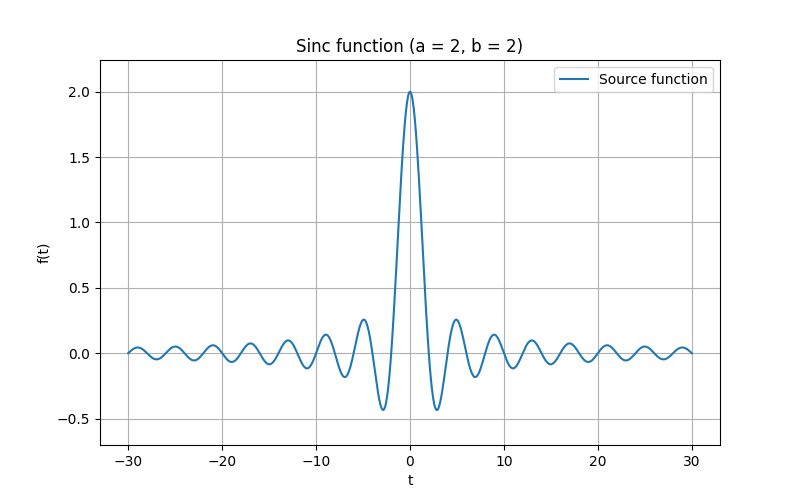
\includegraphics[width=\textwidth]{media/sinc_3.png}
    \caption{График функции $f(t)$ при $a = 2$, $b = 2$}
    \label{fig:sinc_3}
\end{figure}

\FloatBarrier
\subsubsection{Нахождение образа функции}
Согласно формуле \eqref{eq:image_from_function}, Фурье образ функции $f(t)$ задается следующим выражением:

\begin{multline}
    \hat{f}(\omega) = \frac{1}{\sqrt{2\pi}} \int_{-\infty}^{\infty} f(t) e^{-i\omega t} dt = \frac{1}{\sqrt{2\pi}} \int_{-\infty}^{\infty} a \sinc(bt) e^{-i\omega t} dt = \frac{a}{\sqrt{2\pi}} \int_{-\infty}^{\infty} \sinc(bt) e^{-i\omega t} dt = \\
    \frac{1}{\sqrt{2\pi}} \frac{\pi \begin{cases} 0 &, \frac{b^2}{\omega^2} \le 1 \\ 1 & \text{otherwise} \end{cases}}{|b|}
\end{multline}

\subsubsection{Графики образов функций}
Графики образов функции \eqref{eq:sinc_function} при различных значениях $a$ и $b$ представлены на рисунках \ref{fig:sinc_1_image}, \ref{fig:sinc_2_image} и \ref{fig:sinc_3_image}.

\begin{figure}[ht!]
    \centering
    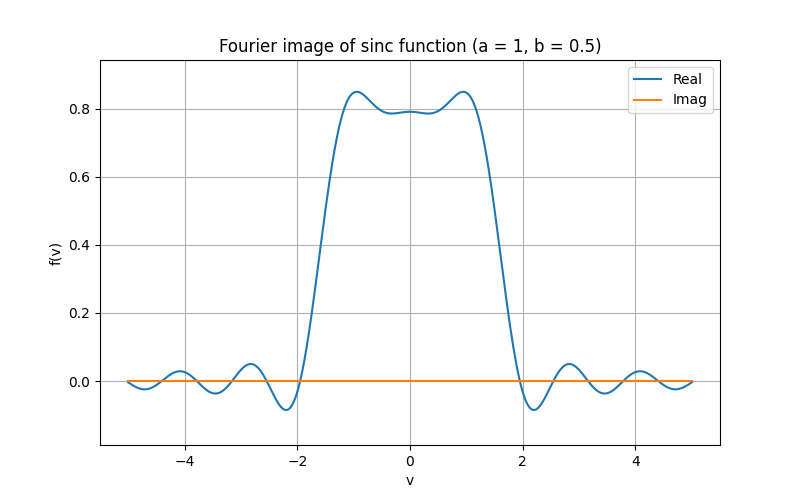
\includegraphics[width=\textwidth]{media/sinc_1_image.png}
    \caption{График образа функции $f(t)$ при $a = 1$, $b = 0.5$}
    \label{fig:sinc_1_image}
\end{figure}

\begin{figure}[ht!]
    \centering
    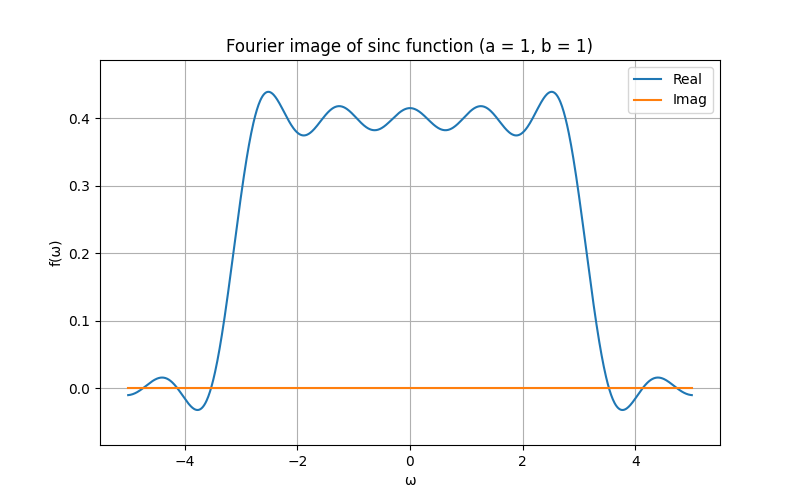
\includegraphics[width=\textwidth]{media/sinc_2_image.png}
    \caption{График образа функции $f(t)$ при $a = 1$, $b = 1$}
    \label{fig:sinc_2_image}
\end{figure}

\begin{figure}[ht!]
    \centering
    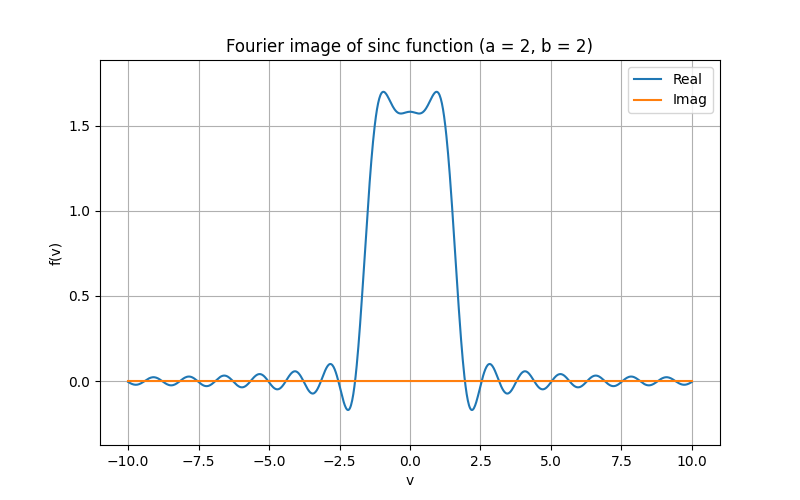
\includegraphics[width=\textwidth]{media/sinc_3_image.png}
    \caption{График образа функции $f(t)$ при $a = 2$, $b = 2$}
    \label{fig:sinc_3_image}
\end{figure}

\FloatBarrier
\subsubsection{Проверка равенства Парсеваля}
Проверим равенство Парсеваля (см. формулу~\eqref{eq:parseval_indentity}). Для этого воспользуемся функцией \texttt{parseval\_check}. 
\begin{table}[ht!]
    \centering
    \begin{tabular}{|c|c|}
        \hline
        $\displaystyle\int_{-100}^{100}{|f(t)|^2}$ & $\displaystyle\int_{-100}^{100}{|\hat{f_1}(\omega)|^2}$ \\
        \hline
        1.9959 & 1.9957 \\
        \hline
    \end{tabular}
    \caption{Результаты проверки равенства Парсеваля для кардинального синуса $f(t)$ при $a = 1$, $b = 0.5$}
    \label{tab:sinc_1_parseval_check}
\end{table}

\begin{table}[ht!]
    \centering
    \begin{tabular}{|c|c|}
        \hline
        $\displaystyle\int_{-100}^{100}{|f(t)|^2}$ & $\displaystyle\int_{-100}^{100}{|\hat{f_2}(\omega)|^2}$ \\
        \hline
        0.9989 & 0.9982 \\
        \hline
    \end{tabular}
    \caption{Результаты проверки равенства Парсеваля для кардинального синуса $f(t)$ при $a = 1$, $b = 1$}
    \label{tab:sinc_2_parseval_check}
\end{table}

\begin{table}[ht!]
    \centering
    \begin{tabular}{|c|c|}
        \hline
        $\displaystyle\int_{-100}^{100}{|f(t)|^2}$ & $\displaystyle\int_{-100}^{100}{|\hat{f_3}(\omega)|^2}$ \\
        \hline
        1.9989 & 1.9996 \\
        \hline
    \end{tabular}
    \caption{Результаты проверки равенства Парсеваля для кардинального синуса $f(t)$ при $a = 2$, $b = 2$}
    \label{tab:sinc_3_parseval_check}
\end{table}

Видим, что во всех случаях равенство Парсеваля выполняется с хорошей точностью. 

\subsubsection{Анализ результатов}
Коэффициент $a$ влияет на амплитуду функции, а коэффициент $b$ влияет на частоту колебаний. При увеличении $a$ амплитуда увеличивается, при увеличении $b$ частота увеличивается.
Видим, что график образа функции похож на график квадратичной функции, это связано с тем, что образ квадратичной функции как раз является кардинальным синусом, а значит, что образ кардинального синуса является квадратичной функцией.

Принцип неопределенности проявляется здесь ровно так же, как и в случае с квадратичной функцией. При уменьшении ширины кардинального синуса увеличивается ширина его образа.  
\FloatBarrier

\subsection{Функция Гаусса}

Рассмотрим семейство функций
\begin{equation}
    f(t) = a e^{-bt^2}
    \label{eq:gaussian_function}
\end{equation}

\subsubsection{Графики исходных функций}
Графики данной функции при различных значениях $a$ и $b$ представлены на рисунках \ref{fig:gaussian_1}, \ref{fig:gaussian_2} и \ref{fig:gaussian_3}.

\begin{figure}[ht!]
    \centering
    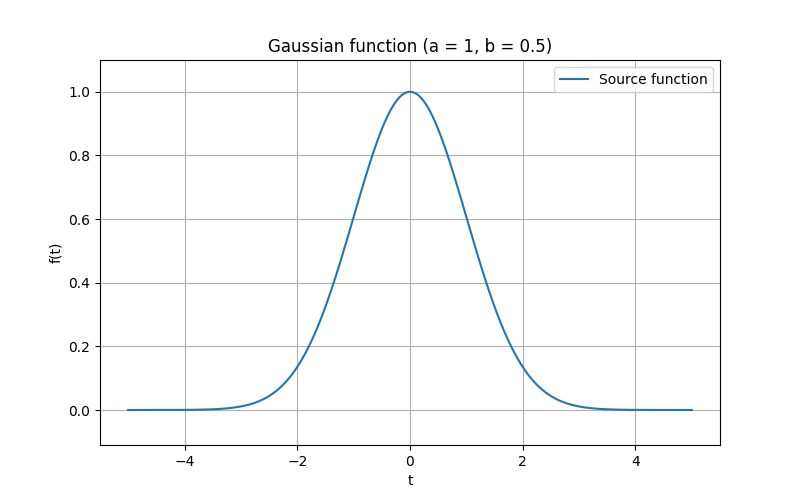
\includegraphics[width=\textwidth]{media/gaussian_1.png}
    \caption{График функции $f(t)$ при $a = 1$, $b = 0.5$}
    \label{fig:gaussian_1}
\end{figure}

\begin{figure}[ht!]
    \centering
    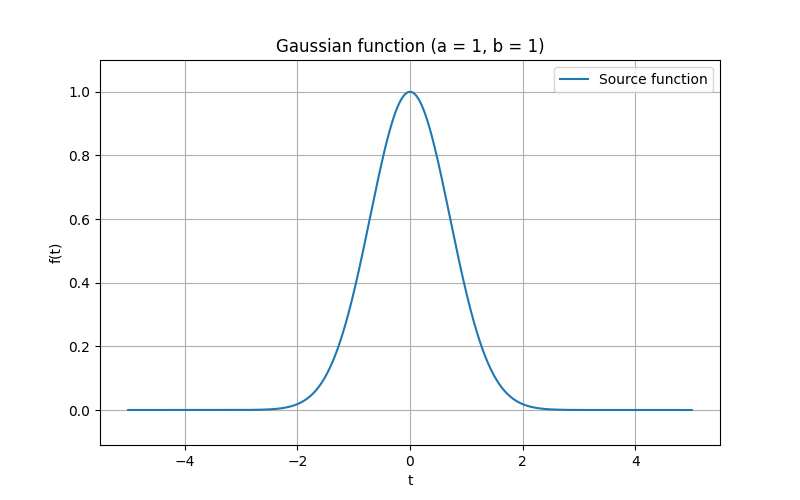
\includegraphics[width=\textwidth]{media/gaussian_2.png}
    \caption{График функции $f(t)$ при $a = 1$, $b = 1$}
    \label{fig:gaussian_2}
\end{figure}

\begin{figure}[ht!]
    \centering
    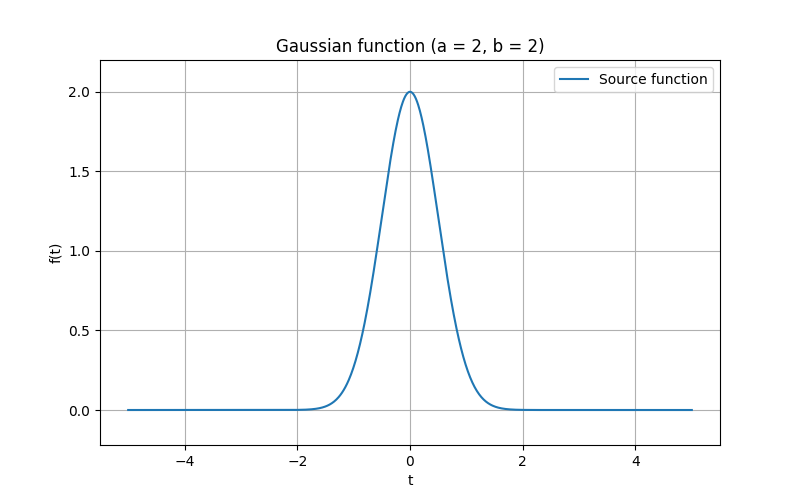
\includegraphics[width=\textwidth]{media/gaussian_3.png}
    \caption{График функции $f(t)$ при $a = 2$, $b = 2$}
    \label{fig:gaussian_3}
\end{figure}

\subsubsection{Нахождение образа функции}
Согласно формуле \eqref{eq:image_from_function}, Фурье образ функции $f(t)$ задается следующим выражением:
\begin{multline}
    \hat{f}(\omega) = \frac{1}{\sqrt{2\pi}} \int_{-\infty}^{\infty} f(t) e^{-i\omega t} dt = \frac{1}{\sqrt{2\pi}} \int_{-\infty}^{\infty} a e^{-bt^2} e^{-i\omega t} dt = \frac{a}{\sqrt{2\pi}} \int_{-\infty}^{\infty} e^{-bt^2} e^{-i\omega t} dt = \\
    \frac{a}{\sqrt{2\pi}} \int_{-\infty}^{\infty} e^{-t(bt +i\omega)} dt = \frac{ae^{\frac{-\omega^2}{4b}}}{\sqrt{2b}}
\end{multline}

\subsubsection{Графики образов функций}
Графики образов функции \eqref{eq:gaussian_function} при различных значениях $a$ и $b$ представлены на рисунках \ref{fig:gaussian_1_image}, \ref{fig:gaussian_2_image} и \ref{fig:gaussian_3_image}.

\begin{figure}[ht!]
    \centering
    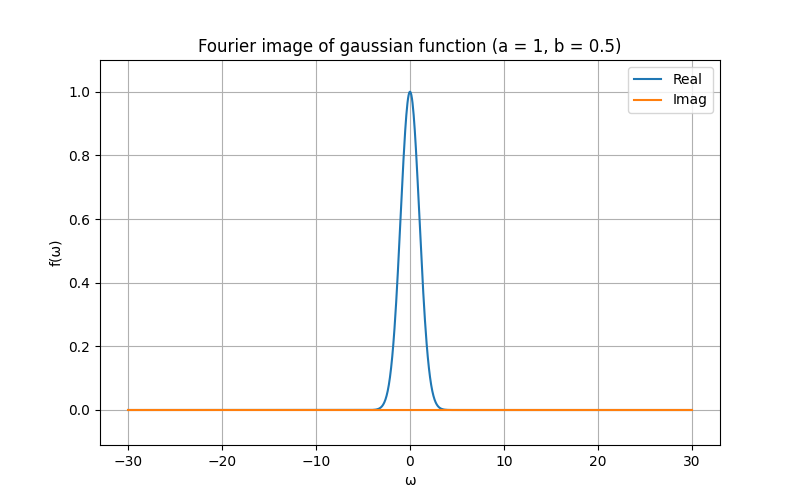
\includegraphics[width=\textwidth]{media/gaussian_1_image.png}
    \caption{График образа функции $f(t)$ при $a = 1$, $b = 0.5$}
    \label{fig:gaussian_1_image}
\end{figure}

\begin{figure}[ht!]
    \centering
    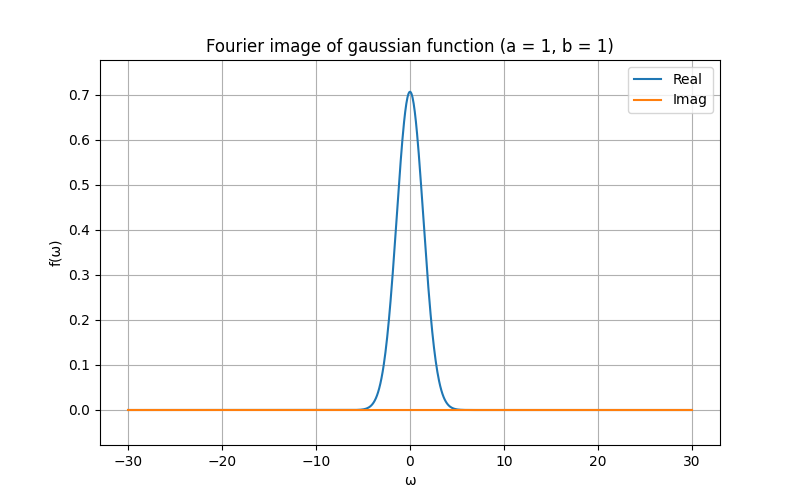
\includegraphics[width=\textwidth]{media/gaussian_2_image.png}
    \caption{График образа функции $f(t)$ при $a = 1$, $b = 1$}
    \label{fig:gaussian_2_image}
\end{figure}

\begin{figure}[ht!]
    \centering
    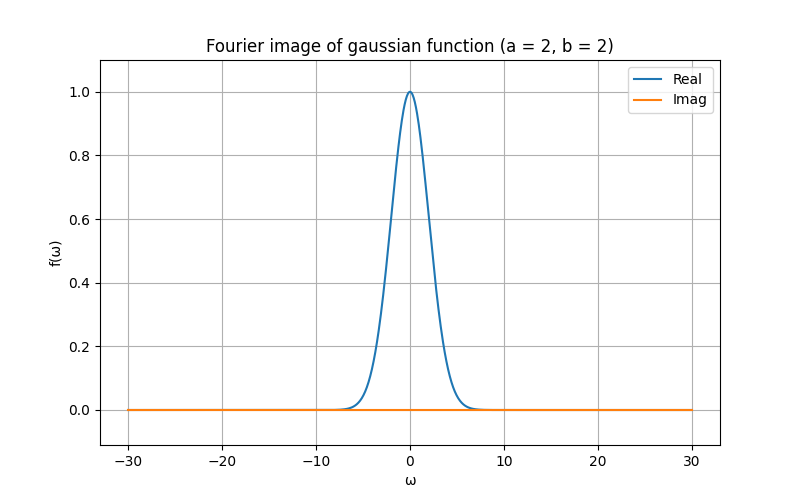
\includegraphics[width=\textwidth]{media/gaussian_3_image.png}
    \caption{График образа функции $f(t)$ при $a = 2$, $b = 2$}
    \label{fig:gaussian_3_image}
\end{figure}

\FloatBarrier
\subsubsection{Провека равенства Парсеваля}
Проверим выполнение равенства Парсеваля для функции \eqref{eq:gaussian_function} при $a = 1$, $b = 1$:
% table with parseval check results
\begin{table}[ht!]
    \centering
    \begin{tabular}{|c|c|}
        \hline
        $\displaystyle\int_{-100}^{100}{|f(t)|^2}$ & $\displaystyle\int_{-100}^{100}{|\hat{f_1}(\omega)|^2}$ \\
        \hline
        1.7724 & 1.7724 \\
        \hline
    \end{tabular}
    \caption{Результаты проверки равенства Парсеваля для функции Гаусса $f(t)$ при $a = 1$, $b = 0.5$}
    \label{tab:gaussian_1_parseval_check}
\end{table}

\begin{table}
    \centering
    \begin{tabular}{|c|c|}
        \hline
        $\displaystyle\int_{-100}^{100}{|f(t)|^2}$ & $\displaystyle\int_{-100}^{100}{|\hat{f_2}(\omega)|^2}$ \\
        \hline
        1.2533 & 1.2533 \\
        \hline
    \end{tabular}
    \caption{Результаты проверки равенства Парсеваля для функции Гаусса $f(t)$ при $a = 1$, $b = 1$}
    \label{tab:gaussian_2_parseval_check}
\end{table}

\begin{table}
    \centering
    \begin{tabular}{|c|c|}
        \hline
        $\displaystyle\int_{-100}^{100}{|f(t)|^2}$ & $\displaystyle\int_{-100}^{100}{|\hat{f_3}(\omega)|^2}$ \\
        \hline
        3.5449 & 3.5449 \\
        \hline
    \end{tabular}
    \caption{Результаты проверки равенства Парсеваля для функции Гаусса $f(t)$ при $a = 2$, $b = 2$}
    \label{tab:gaussian_3_parseval_check}
\end{table}

Видим, что равенство Парсеваля выполняется для всех значений $a$ и $b$ с точностью до способа вычисления интегралов.

\subsubsection{Анализ результатов}
Влияние параметров $a$ и $b$ на функцию Гаусса можно понять по формулам \eqref{eq:gaussian_function} и \eqref{eq:image_from_function}. Параметр $a$ отвечает за амплитуду функции, а параметр $b$ за ширину исходной функция. При увеличении $a$ амплитуда функции увеличивается, при увеличении $b$ функция становится уже. 
Эти выводы подтверждаются графиками исходной функции и ее образа.
\FloatBarrier

\subsection{Двустороннее затухание}

Рассмотрим семейство функций 
\begin{equation}
    f(t) = ae^{-b|t|}
    \label{eq:fade_function}
\end{equation}

\subsubsection{Графики исходных функций}

Графики данной функции при различных значениях $a$ и $b$ представлены на рисунках \ref{fig:fade_1}, \ref{fig:fade_2} и \ref{fig:fade_3}.
\begin{figure}[ht!]
    \centering
    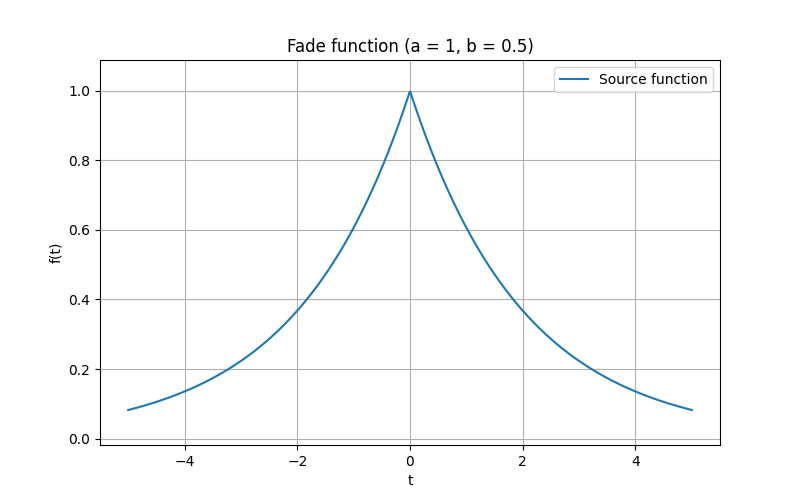
\includegraphics[width=\textwidth]{media/fade_1.png}
    \caption{График функции $f(t)$ при $a = 1$, $b = 0.5$}
    \label{fig:fade_1}
\end{figure}

\begin{figure}[ht!]
    \centering
    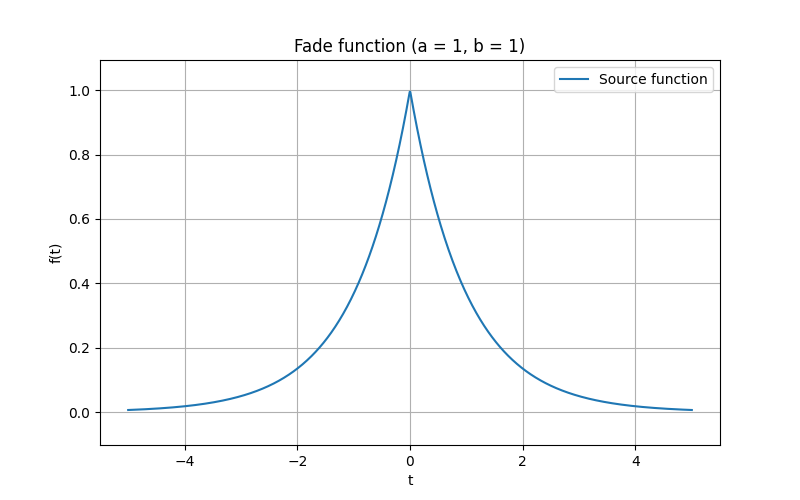
\includegraphics[width=\textwidth]{media/fade_2.png}
    \caption{График функции $f(t)$ при $a = 1$, $b = 1$}
    \label{fig:fade_2}
\end{figure}

\begin{figure}[ht!]
    \centering
    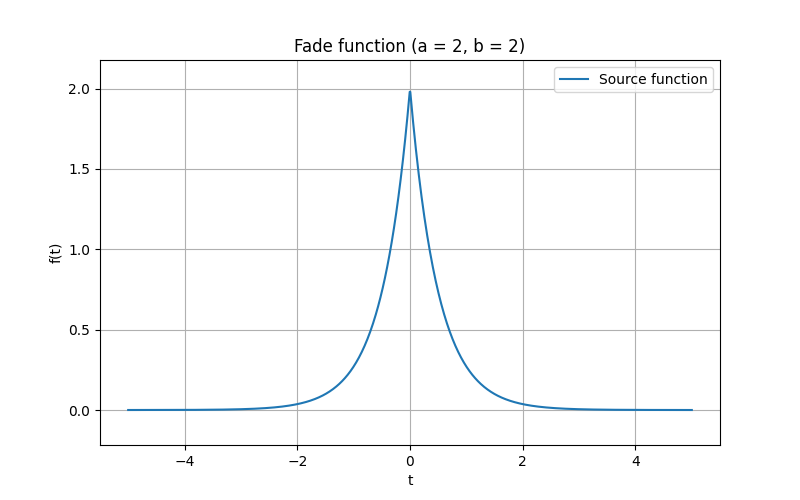
\includegraphics[width=\textwidth]{media/fade_3.png}
    \caption{График функции $f(t)$ при $a = 2$, $b = 2$}
    \label{fig:fade_3}
\end{figure}

\subsubsection{Нахождение образа функции}
Согласно формуле \eqref{eq:image_from_function}, Фурье образ функции $f(t)$ задается следующим выражением:
\begin{multline}
    \hat{f}(\omega) = \frac{1}{\sqrt{2\pi}} \int_{-\infty}^{\infty} f(t) e^{-i\omega t} dt = \frac{1}{\sqrt{2\pi}} \left(\int_{-\infty}^{0} ae^{bt} e^{-i\omega t} dt + \int_{0}^{\infty} ae^{-bt} e^{-i\omega t} dt\right) = \\
    \frac{a}{\sqrt{2\pi}} \left(\int_{-\infty}^0 e^{t(b -i \omega)}dt + \int_0^{\infty} e^{t(-b - i\omega)}dt\right) = \frac{a}{\sqrt{2 \pi}} \left( \frac{1}{b - i\omega} + \frac{1}{b + i\omega}\right) = \frac{\sqrt{2/\pi}ab}{b^2 + \omega^2}
    \label{eq:fade_function_image}
\end{multline}

\subsubsection{Графики образов функций}
Графики образов функции при различных значениях $a$ и $b$ представлены на рисунках \ref{fig:fade_1_image}, \ref{fig:fade_2_image} и \ref{fig:fade_3_image}.

\begin{figure}[ht!]
    \centering
    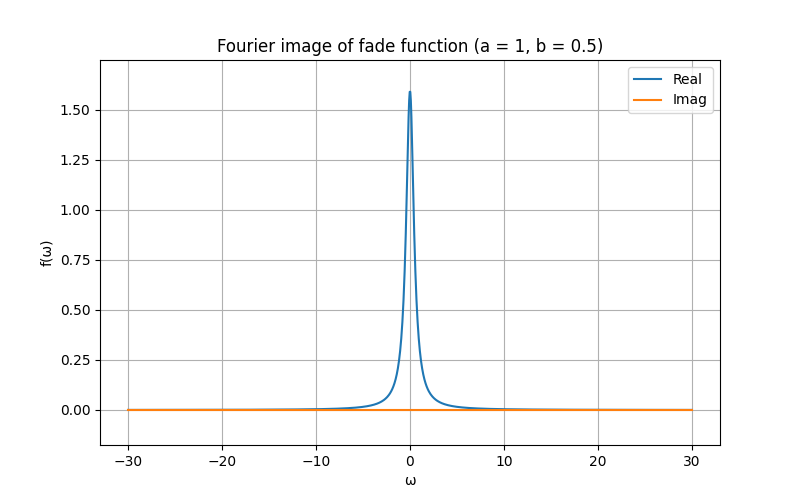
\includegraphics[width=\textwidth]{media/fade_1_image.png}
    \caption{График образа функции $f(t)$ при $a = 1$, $b = 0.5$}
    \label{fig:fade_1_image}
\end{figure}

\begin{figure}[ht!]
    \centering
    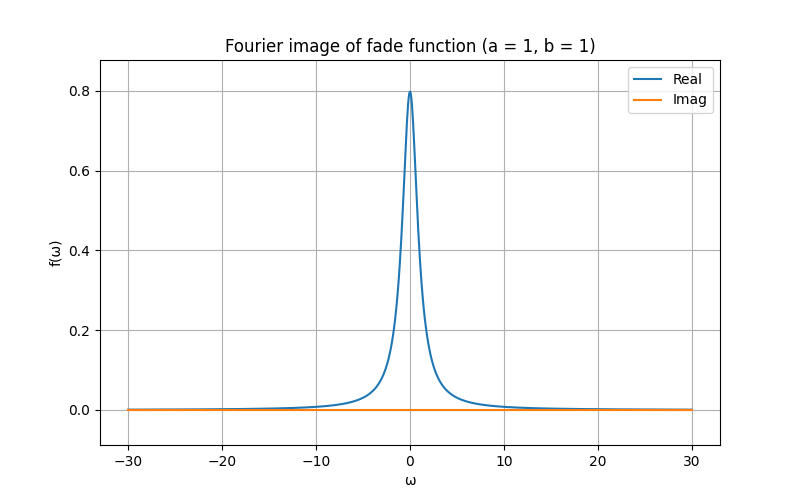
\includegraphics[width=\textwidth]{media/fade_2_image.png}
    \caption{График образа функции $f(t)$ при $a = 1$, $b = 1$}
    \label{fig:fade_2_image}
\end{figure}

\begin{figure}[ht!]
    \centering
    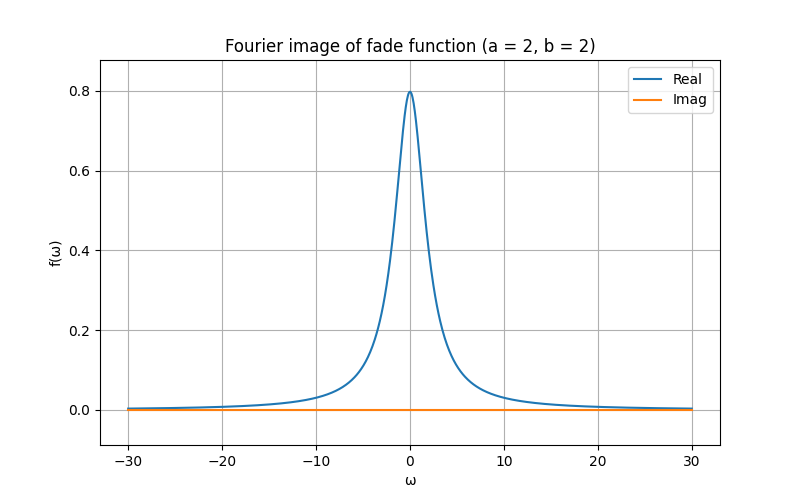
\includegraphics[width=\textwidth]{media/fade_3_image.png}
    \caption{График образа функции $f(t)$ при $a = 2$, $b = 2$}
    \label{fig:fade_3_image}
\end{figure}

\FloatBarrier
\subsubsection{Проверка равенства Парсеваля}
Проверим равенство Парсеваля (см. формулу~\eqref{eq:parseval_indentity}). Для этого воспользуемся функцией \texttt{parseval\_check}.
% table with parseval check results
\begin{table}[ht!]
    \centering
    \begin{tabular}{|c|c|}
        \hline
        $\displaystyle\int_{-100}^{100}{|f(t)|^2}$ & $\displaystyle\int_{-100}^{100}{|\hat{f_1}(\omega)|^2}$ \\
        \hline
        1.9998 & 1.9998 \\
        \hline
    \end{tabular}
    \caption{Результаты проверки равенства Парсеваля для функции затухания $f(t)$ при $a = 1$, $b = 0.5$}
    \label{tab:fade_1_parseval_check}
\end{table}

\begin{table}[ht!]
    \centering
    \begin{tabular}{|c|c|}
        \hline
        $\displaystyle\int_{-100}^{100}{|f(t)|^2}$ & $\displaystyle\int_{-100}^{100}{|\hat{f_2}(\omega)|^2}$ \\
        \hline
        0.9997 & 0.9997 \\
        \hline
    \end{tabular}
    \caption{Результаты проверки равенства Парсеваля для функции затухания $f(t)$ при $a = 1$, $b = 1$}
    \label{tab:fade_2_parseval_check}
\end{table}

\begin{table}[ht!]
    \centering
    \begin{tabular}{|c|c|}
        \hline
        $\displaystyle\int_{-100}^{100}{|f(t)|^2}$ & $\displaystyle\int_{-100}^{100}{|\hat{f_3}(\omega)|^2}$ \\
        \hline
        1.9978 & 1.9978 \\
        \hline
    \end{tabular}
    \caption{Результаты проверки равенства Парсеваля для функции затухания $f(t)$ при $a = 2$, $b = 2$}
    \label{tab:fade3_parseval_check}
\end{table}

Видим, что во всех случаях значения почти не отличаются друг от друга. Различие, по большей части, обусловлено тем, что в программе нельзя найти интеграл по бесконечности, поэтому просто берется достаточно большой интервал интегрирования.

\subsubsection{Анализ результатов}
Влияние параметров $a$ и $b$ на графики функции и ее образа можно описать следующим образом, в соответствиями с формулами \eqref{eq:fade_function} и \eqref{eq:fade_function_image}: $a$ отвечает за амплитуду функции, а $b$ за скорость затухания. При увеличении $a$ амплитуда функции увеличивается, а при увеличении $b$ функция затухает быстрее. 

\FloatBarrier

\section{Комплексная функция}
\subsection{Сдвинутая прямоугольная функция}
Рассмотрим прямоугольную функция из первого задания (см. формулу~\eqref{eq:rectangle_function}). Примем $a = 1$, $b = 0.5$. 
Рассмотрим \textit{сдвинутую функцию} $g(t) = f(t + c)$

\subsubsection{Графики исходных функции}
Графики данной функции при различных значениях $c$ представлены на рисунках \ref{fig:moved_rectangle_1}, \ref{fig:moved_rectangle_2} и \ref{fig:moved_rectangle_3}.

\begin{figure}[ht!]
    \centering
    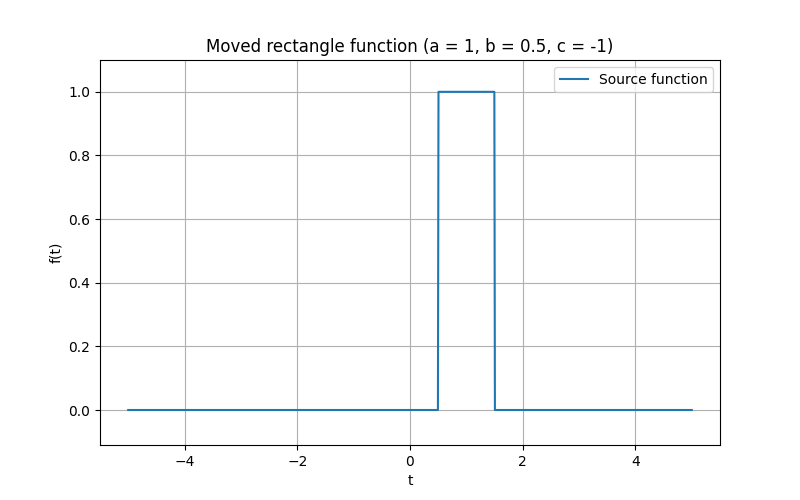
\includegraphics[width=\textwidth]{media/moved_rectangle_1.png}
    \caption{График функции $g(t)$ при $c = -1$}
    \label{fig:moved_rectangle_1}
\end{figure}

\begin{figure}[ht!]
    \centering
    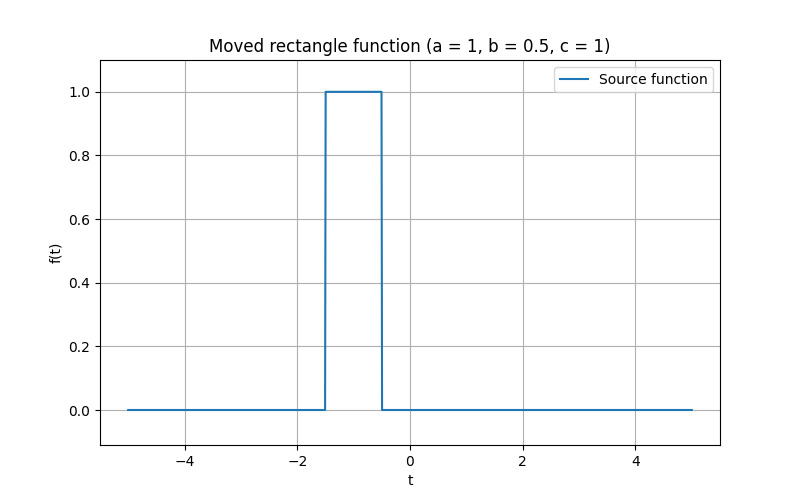
\includegraphics[width=\textwidth]{media/moved_rectangle_2.png}
    \caption{График функции $g(t)$ при $c = 1$}
    \label{fig:moved_rectangle_2}
\end{figure}

\begin{figure}[ht!]
    \centering
    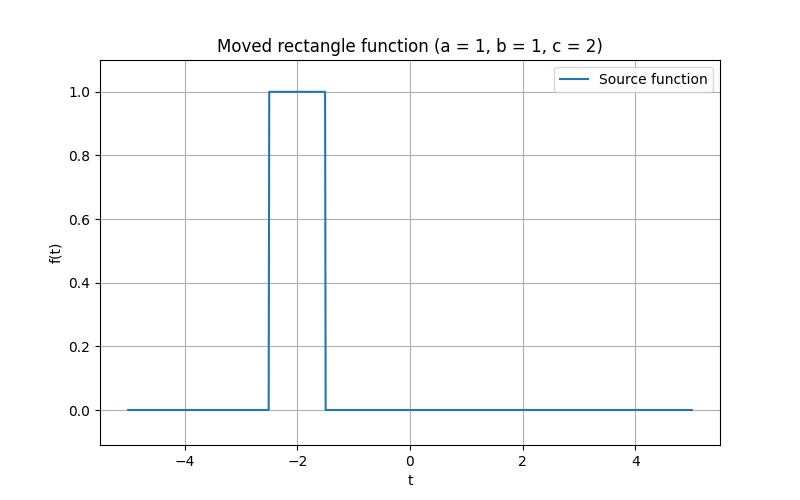
\includegraphics[width=\textwidth]{media/moved_rectangle_3.png}
    \caption{График функции $g(t)$ при $c = 2$}
    \label{fig:moved_rectangle_3}
\end{figure}
\FloatBarrier

\subsubsection{Нахождение образа функции}

Согласно формуле \eqref{eq:image_from_function}, Фурье образ функции $g(t)$ задается следующим выражением:
\begin{multline}
    \hat{g}(\omega) = \frac{1}{\sqrt{2\pi}} \int_{-\infty}^{\infty} g(t) e^{-i\omega t} dt = \frac{1}{\sqrt{2\pi}} \int_{-\infty}^{\infty} f(t + c) e^{-i\omega t} dt = \frac{1}{\sqrt{2\pi}} \int_{-\infty}^{\infty} f(t) e^{-i\omega (t - c)} dt = \\
    \frac{1}{\sqrt{2\pi}} \int_{-b}^{b} a e^{-i\omega (t - c)} d(t - c) = \frac{a}{-\omega i\sqrt{2\pi}} e^{-i\omega (t - c)} \Biggr|_{-b}^{b} = \frac{a(e^{i\omega (b + c)} - e^{-i\omega (b - c)})}{\omega i \sqrt{2 \pi}} = \frac{a e^{i\omega c} (e^{i\omega b} - e^{-i\omega b})}{\omega i \sqrt{2\pi}} =\\
    \frac{2ae^{i\omega c} \sin{\omega b}}{\omega \sqrt{2\pi}} = \frac{2abe^{i\omega c}}{\sqrt{2\pi}}\sinc{\omega b}
    \label{eq:moved_rectangle_image}
\end{multline}

Заметим, что относительно прошлого образа функции (см. формулу~\eqref{eq:rectangle_image}) добавился множитель $e^{i\omega c}$. Он отвечает за \textit{поворот} образа в комплексной плоскости. Таким образом, образ сдвинутой функции является комплексным. 

\subsubsection{Графики образов функций}
Графики образов функции при различных значениях $c$ представлены на рисунках \ref{fig:moved_rectangle_1_image}, \ref{fig:moved_rectangle_2_image} и \ref{fig:moved_rectangle_3_image}.

\begin{figure}[ht!]
    \centering
    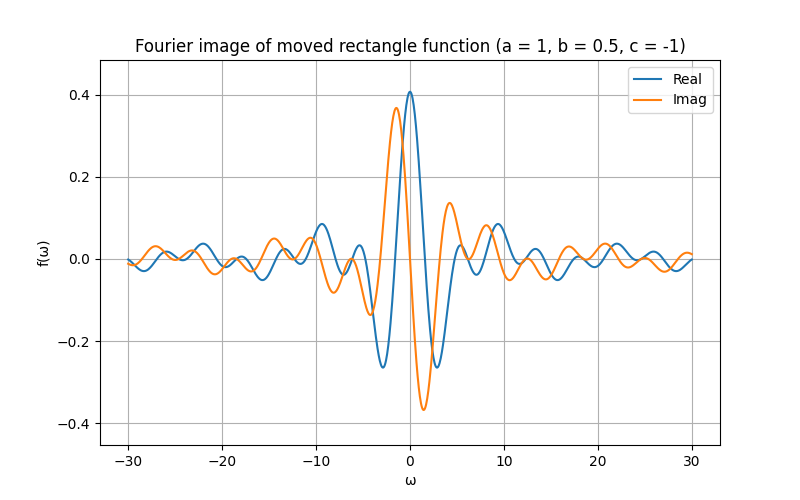
\includegraphics[width=\textwidth]{media/moved_rectangle_1_image.png}
    \caption{График образа функции $g(t)$ при $c = -1$}
    \label{fig:moved_rectangle_1_image}
\end{figure}

\begin{figure}[ht!]
    \centering
    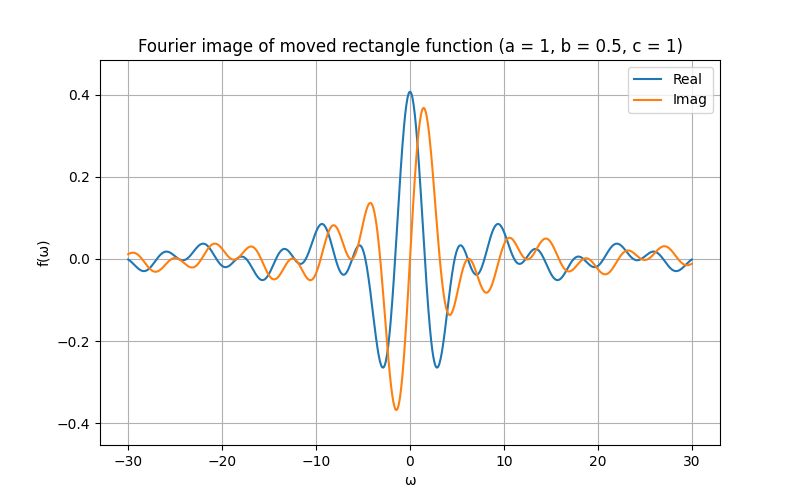
\includegraphics[width=\textwidth]{media/moved_rectangle_2_image.png}
    \caption{График образа функции $g(t)$ при $c = 1$}
    \label{fig:moved_rectangle_2_image}
\end{figure}

\begin{figure}[ht!]
    \centering
    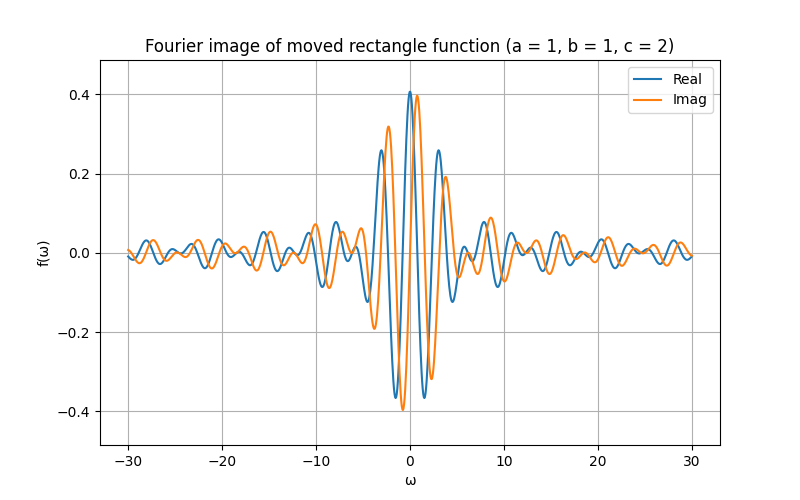
\includegraphics[width=\textwidth]{media/moved_rectangle_3_image.png}
    \caption{График образа функции $g(t)$ при $c = 2$}
    \label{fig:moved_rectangle_3_image}
\end{figure}

Кроме того, рассмотрим графики модуля образа функции на рисунках \ref{fig:moved_rectangle_1_image_abs}, \ref{fig:moved_rectangle_2_image_abs} и \ref{fig:moved_rectangle_3_image_abs}.

\begin{figure}[ht!]
    \centering
    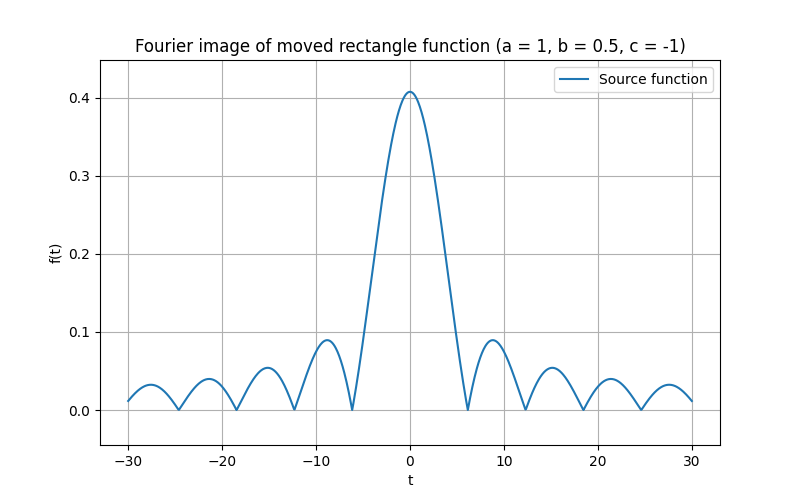
\includegraphics[width=\textwidth]{media/moved_rectangle_1_image_abs.png}
    \caption{График модуля образа функции $g(t)$ при $c = -1$}
    \label{fig:moved_rectangle_1_image_abs}
\end{figure}

\begin{figure}[ht!]
    \centering
    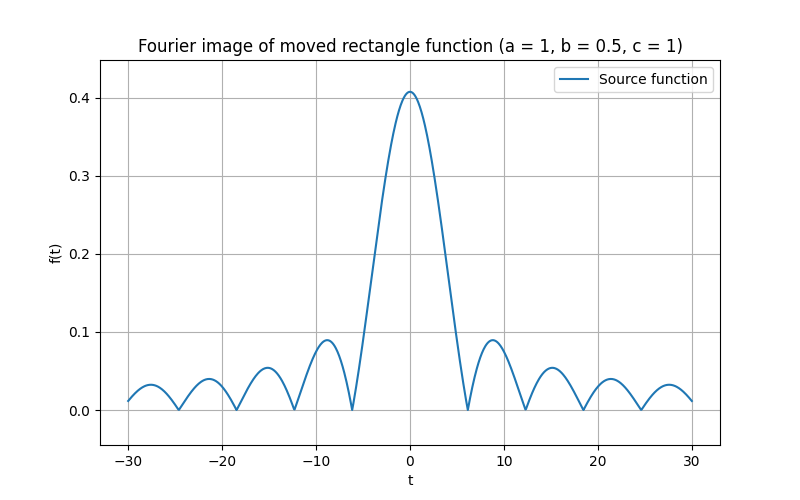
\includegraphics[width=\textwidth]{media/moved_rectangle_2_image_abs.png}
    \caption{График модуля образа функции $g(t)$ при $c = 1$}
    \label{fig:moved_rectangle_2_image_abs}
\end{figure}

\begin{figure}[ht!]
    \centering
    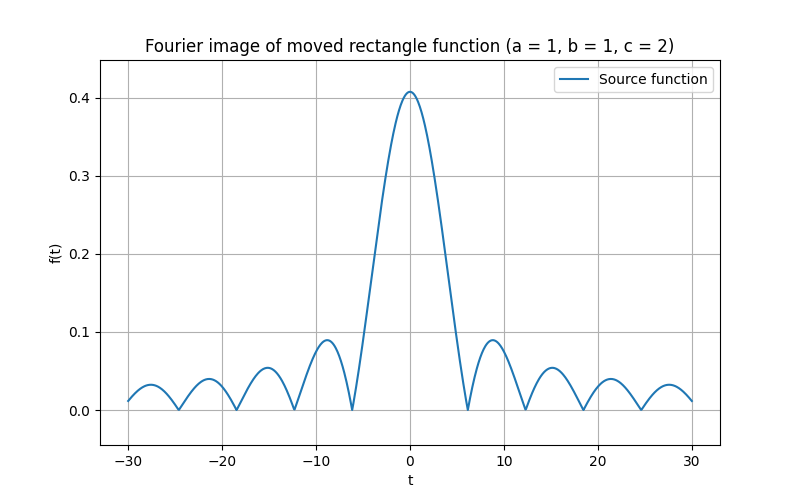
\includegraphics[width=\textwidth]{media/moved_rectangle_3_image_abs.png}
    \caption{График модуля образа функции $g(t)$ при $c = 2$}
    \label{fig:moved_rectangle_3_image_abs}
\end{figure}

Видим, что графики модуля образа функции не отличаются в зависимости от значения $c$. Это связано с тем, что модуль комплексного числа не зависит от его аргумента.

\FloatBarrier

\subsubsection{Проверка равенства Парсеваля}
Проверим равенство Парсеваля (см. формулу~\eqref{eq:parseval_indentity}). Для этого воспользуемся функцией \texttt{parseval\_check}. 

\begin{table}[ht!]
    \centering
    \begin{tabular}{|c|c|}
        \hline
        $\displaystyle\int_{-100}^{100}{|g(t)|^2}$ & $\displaystyle\int_{-100}^{100}{|\hat{g_1}(\omega)|^2}$ \\
        \hline
        1.0010 & 0.9946 \\
        \hline
    \end{tabular}
    \caption{Результаты проверки равенства Парсеваля для сдвинутой прямоугольной функции $g(t)$ при $a = 1$, $b = 0.5, c = -1$}
    \label{tab:moved_rectangle_1_parseval_check}
\end{table}

\begin{table}[ht!]
    \centering
    \begin{tabular}{|c|c|}
        \hline
        $\displaystyle\int_{-100}^{100}{|g(t)|^2}$ & $\displaystyle\int_{-100}^{100}{|\hat{g_2}(\omega)|^2}$ \\
        \hline
        1.00100 & 0.9946 \\
        \hline
    \end{tabular}
    \caption{Результаты проверки равенства Парсеваля для сдвинутой прямоугольной функции $g(t)$ при $a = 1$, $b = 0.5, c = 1$}
    \label{tab:moved_rectangle_2_parseval_check}
\end{table}

\begin{table}[ht!]
    \centering
    \begin{tabular}{|c|c|}
        \hline
        $\displaystyle\int_{-100}^{100}{|g(t)|^2}$ & $\displaystyle\int_{-100}^{100}{|\hat{g_3}(\omega)|^2}$ \\
        \hline
        0.5005 & 0.49417 \\
        \hline
    \end{tabular}
    \caption{Результаты проверки равенства Парсеваля для сдвинутой прямоугольной функции $g(t)$ при $a = 1$, $b = 0.5, c = 2$}
    \label{tab:moved_rectangle_3_parseval_check}
\end{table}
Видим, что полученные значения практически равны. Разница, как и в случае с \textit{не сдвинутыми} функциями обусловлена интегрированием не по всей числовой прямой, а лишь по ее части.

\subsubsection{Анализ результатов}
Видим, что при увеличении значения $c$ график исходной функции, очевидно, сдвигается, а график ее образа \textit{сжимается}, при этом амплитуда остается неизменной. 

\section{Анализ аккорда}
\subsection{Аккорд 23}

Для обработки мною был выбран аккорд номер 23. 

\subsubsection{Графики иходной записи}

График зависимости уровня громкости от времени для исходной записи представлен на рисунке~\ref{fig:waveform}.

\begin{figure}[ht!]
    \centering
    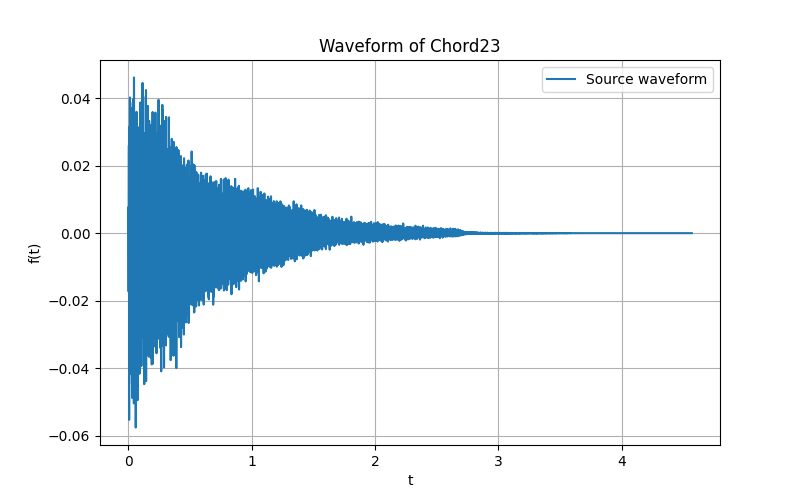
\includegraphics[width=\textwidth]{media/waveform.png}
    \caption{График зависимости уровня громкости от времени для исходной записи}
    \label{fig:waveform}
\end{figure}

Данный график обрезан по времени до 2 секунд, так как далее уровень громкости практически не изменяется.

\subsubsection{Фурье преобразование}
Теперь посмотрим на график образа данной записи в частотной области. Для этого применим к исходной записи преобразование Фурье. График зависимости уровня громкости от частоты представлен на рисунке~\ref{fig:wave_image}.

\begin{figure}[ht!]
    \centering
    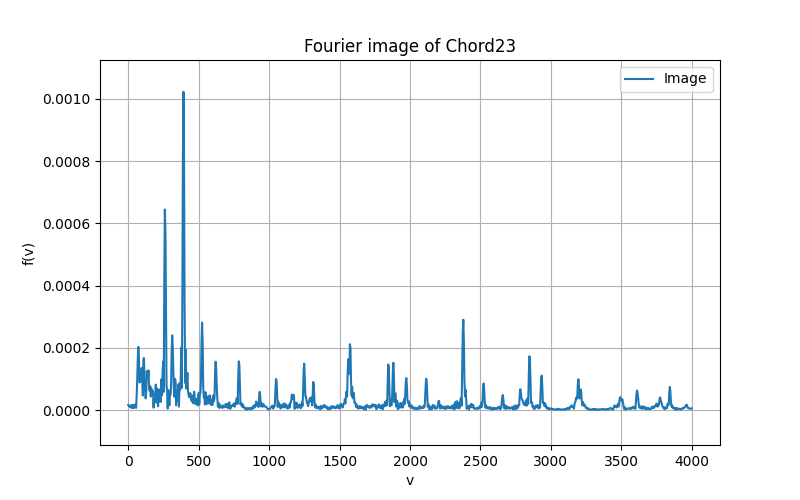
\includegraphics[width=\textwidth]{media/wave_image.png}
    \caption{График зависимости уровня громкости от частоты для исходной записи}
    \label{fig:wave_image}
\end{figure}

Для Нахождения образа использовались первые 0.1 секунда записи для того, чтобы график был более наглядным. На графики представлены частоты от 0 до 4000 Гц. 

\subsubsection{Анализ звуков}
На графике \ref{fig:wave_image} заметны явные пики, которые соответствуют доминирующим частотам. Наиболее выраженные пики находятся на частотах 262 Гц, 311 Гц и 392 Гц, что соответствует нотам C, D\# и G соответственно. Таким образом, исходный аккорд -- \textbf{До минор}. 
\FloatBarrier


